\subsection{Physics of $\mathrm{\gamma \gamma}$ interactions in heavy-ion collisions}
\label{sec:upc}
%%%%%%%%%%%%%%%%%%%%%%%%%%%%%%%%%%%%%%%%%%%%%%%%%%%%%%%%%%%%%%%%%%%%%%

{ \small
\noindent \textbf{Coordinators}: Iwona Grabowska-Bold (AGH UST, Krak\'ow)\\

\noindent \textbf{Contributors}: 
M.~Dyndal (DESY), 
S.~Hassani (Universit\'e Paris-Saclay), 
M.~Klusek-Gawenda (IFJ PAN, PL-31342 Krak\'ow, Poland), 
L.~Schoeffel (Universit\'e Paris-Saclay), Peter Steinberg (BNL)
}

Heavy-ion beams are composed of nuclei which carry electric charge $Ze$~($e$ is the electron charge and $Z$ is the atomic number). They are accelerated to nearly the speed of light, thus they generate extremely large electromagnetic~(EM) fields. 
The EM fields generated by the relativistic ion can interact with the other nucleus or its EM fields.
Therefore, besides nuclear hadronic interactions, EM
interactions also occur in ultra-relativistic heavy-ion collisions.
These EM interactions can be studied in so-called ultra-peripheral
collisions~(UPC) which occur when the distance between two nuclei in the transverse plane is larger than two times the nuclear radius, and hadronic interactions are thus suppressed~\cite{Bertulani:2005ru}.

A broad range of processes can be studied with $\mathrm{\gamma\gamma}$ interactions in UPC. In the following, a few examples of photon-induced processes are considered at the HL-LHC: exclusive production of $\mathrm{\mu^+\mu^-}$ or p$\mathrm{\bar{p}}$ pairs, a rare process of light-by-light~(LbyL) scattering and a potential of searches for axion-like particles~(ALP).

%-------------------------------------------------------------------
\begin{figure}[!hbt]
\centering
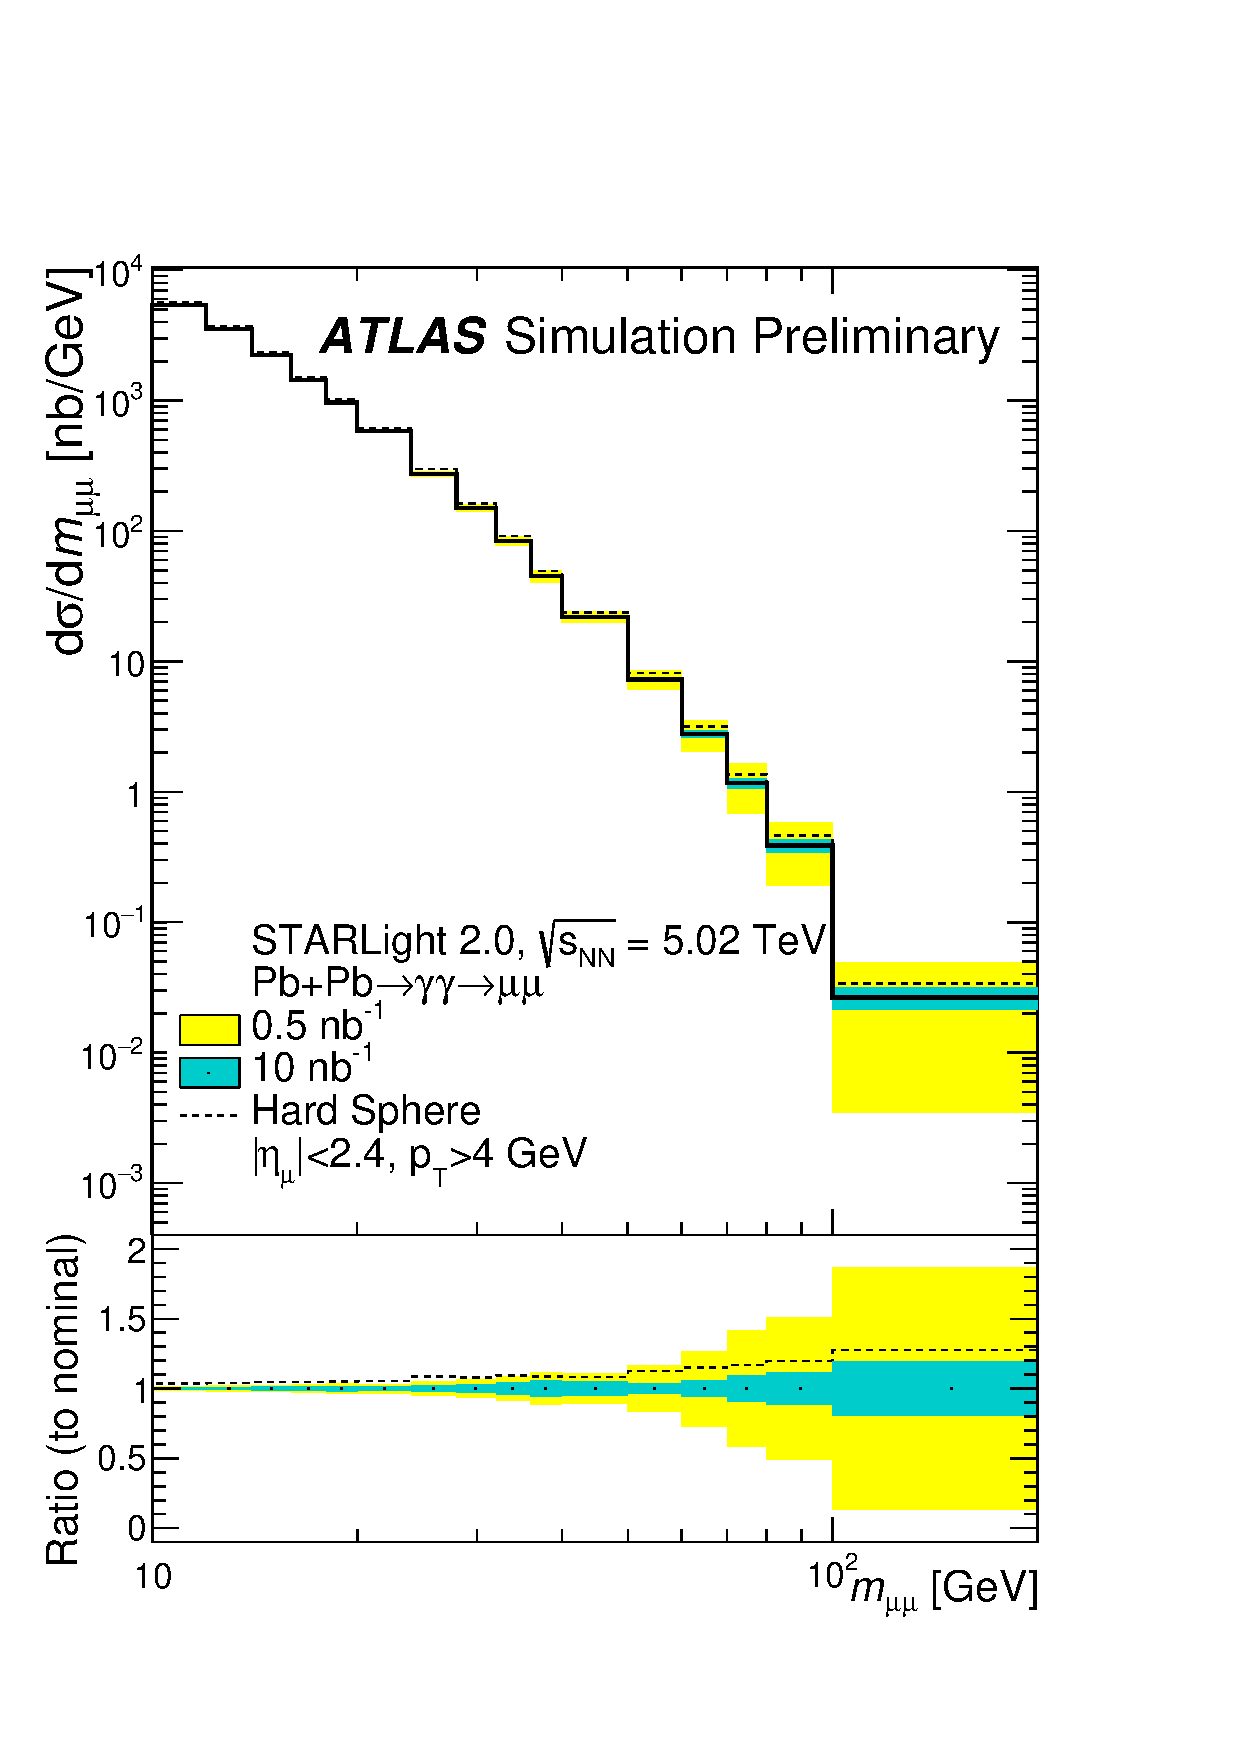
\includegraphics[width=0.50\linewidth]{\main/beyond/fig/fig_01.pdf}
\caption{
(Upper)~Differential cross section for exclusive production of the di-muon pairs as a function of the di-muon mass for
$10<m_{\mathrm{\mu\mu}}<200$~GeV extracted from STARLight. Two
scenarios are considered for the nuclear geometry: a realistic skin
depth of the nucleus~(solid line) or a hard sphere~(dashed
line). (Bottom)~Ratio to nominal as a function of the di-muon mass,
where "nominal'' stands for the realistic skin depth of the nucleus.
 Shaded bands represent expected statistical uncertainties associated with a number of signal events in each bin for integrated luminosity of $0.5~\mathrm{nb}^{-1}$~(yellow), and $10~\mathrm{nb}^{-1}$~(cyan).}
\label{fig:mumu}
\end{figure}
%-------------------------------------------------------------------

Exclusive production of di-muon pairs~($\mathrm{\gamma\gamma\rightarrow \mu^+\mu^-}$) in UPC can offer a precision measurement of photon fluxes associated with ion beams, and as such can be used to constrain predictions for the other processes covered in this section. The cross section at high pair mass is also sensitive to the nuclear geometry assumed in the calculations. Figure~\ref{fig:mumu} presents a differential cross section as a function of the invariant mass of the di-muon system in the range of 10-200~GeV with expected statistical uncertainties represented by two bands corresponding to integrated luminosities of $0.5~\mathrm{nb}^{-1}$ and
$10~\mathrm{nb}^{-1}$. Two scenarios are considered for the nuclear
geometry: a realistic skin depth of the nucleus or a hard sphere~\cite{Barrett:1977}.
For the $10~\mathrm{nb}^{-1}$ scenario, a significant reduction of the
statistical uncertainty is expected for the highest $m_{\mathrm{\mu\mu}}$ bin which spans 100-200~GeV.  This will help in reducing uncertainties from the modelling of the nuclear geometry.
The expected upgrades of the ATLAS Zero Degree Calorimeters~(ZDC) in the LHC Run 3 will also be important for isolating the contributions to the cross section stemming from dissociative processes.

Exclusive production of p$\mathrm{\bar{p}}$ pairs~($\mathrm{\gamma\gamma\rightarrow p\bar{p}}$) in heavy-ion collisions is considered as a process which can help verify the existing theoretical approaches. It has been demonstrated that the existing $\mathrm{\gamma\gamma\rightarrow p\bar{p}}$ experimental data~\cite{Kuo:2005nr} from the Belle Collaboration can be successfully described by implementation of several components~\cite{Klusek-Gawenda:2017lgt}: the non-resonant proton exchange, $s$-channel tensor meson exchange and the hand-bag model~\cite{Diehl:2002yh}. Figure~\ref{fig:ppbar} shows distributions of invariant mass of the p$\mathrm{\bar{p}}$ system, $W_{\mathrm{\gamma\gamma}} = M_{\mathrm{p\bar{p}}}$~(left panel) and of the difference of rapidities for protons and anti-protons, $y_{\mathrm{diff}} = y_\mathrm{p} - y_{\mathrm{\bar{p}}}$~(right panel).
The ALICE Collaboration can measure p$\mathrm{\bar{p}}$ pairs in Pb--Pb collisions at mid-rapidity~($|y|$ < 0.9). 
The LHCb Collaboration could also provide a complementary measurement of p$\mathrm{\bar{p}}$ production in the forward region~(2 <$\eta$ < 4.5).
The upgraded charged particle tracking capabilities of ATLAS and CMS experiments for Run~4 will measure in $|y|<4.0$.
Corresponding kinematic requirements on transverse momenta and rapidity or pseudorapidity specific for each experiment are presented in the figure legend. The calculations are made for Pb--Pb collisions with $\sqrt{s_{\mathrm{NN}}}$ = 5.52~TeV.
The total cross section predicted for the ATLAS and CMS acceptance for $\pt>0.2$~GeV~($\pt>0.5$~GeV) is $\sigma$ = 793~$\mu$b~(248~$\mu$b), while LHCb and ALICE requirements lead to $\sigma$ = 125 and 105~$\mu$b, respectively.

%-------------------------------------------------------------------
\begin{figure}[!h]
        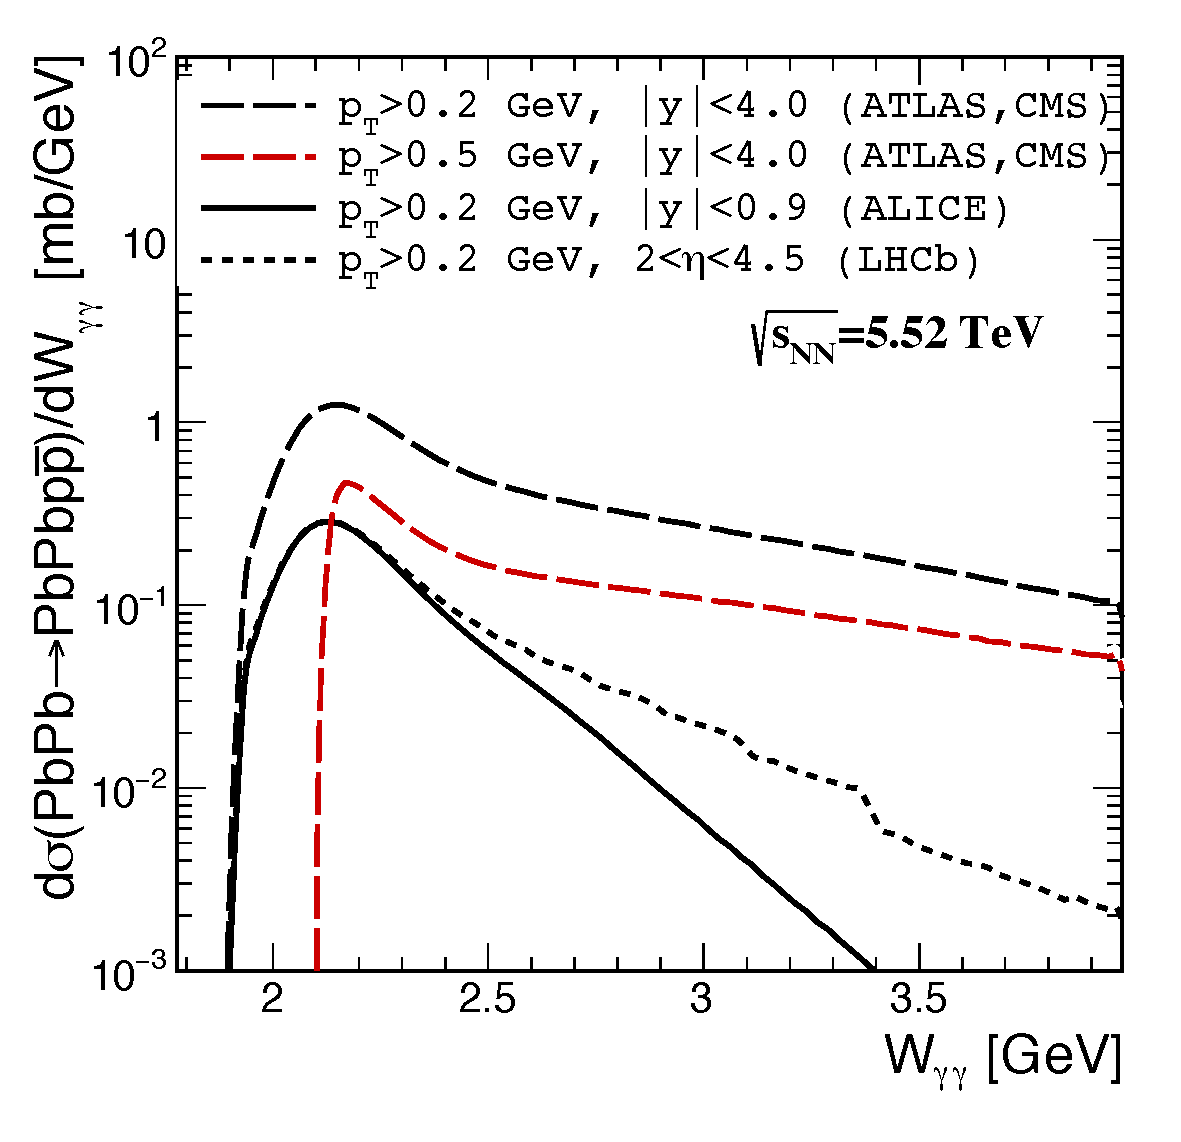
\includegraphics[scale=0.375]{\main/beyond/fig/dsig_dw_4exp_plus_y4_nucl_5520GeV.pdf}
        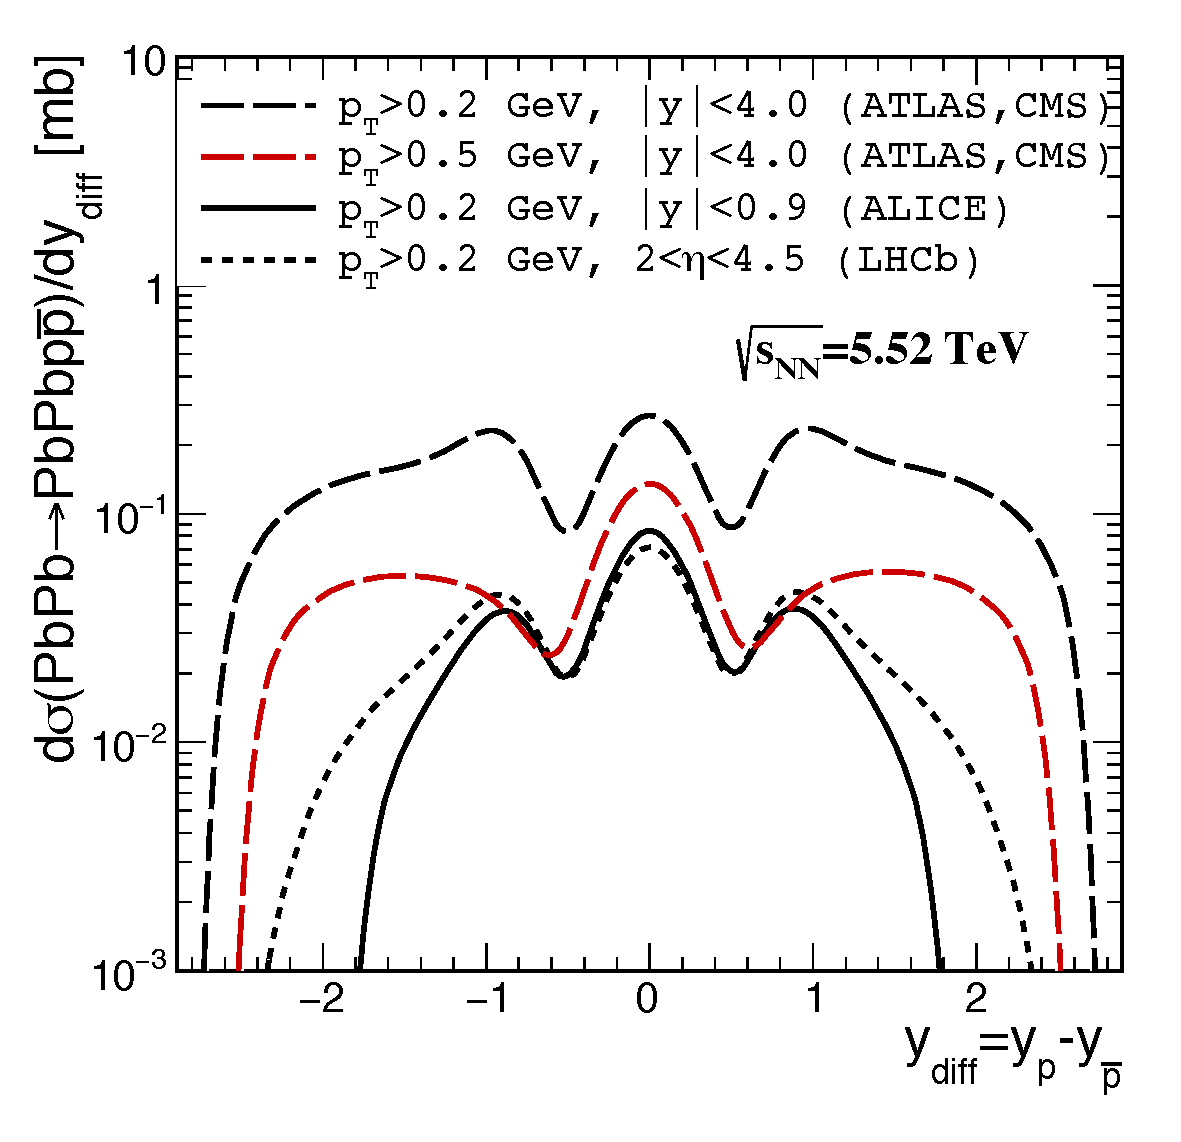
\includegraphics[scale=0.375]{\main/beyond/fig/dsig_dydiff_4exp_plus_y4_nucl_5520GeV.pdf}
        \caption{
                Differential cross sections as a function of $\mathrm{p\bar{p}}$
                invariant mass~(left) and rapidity
                distance between proton and anti-proton~(right)
                in Pb--Pb collisions at $\sqrt{s_{\mathrm{NN}}}$=5.52\,TeV
                for four experimental acceptance requirements. 
                For ATLAS and CMS experiments two requirements for proton $\pt>0.2$~GeV or $\pt>0.5$~GeV are considered.
        }
        \label{fig:ppbar}
\end{figure}
%-------------------------------------------------------------------


From the left panel of Figure~\ref{fig:ppbar} one can deduce that the dependence on invariant mass of the $\mathrm{p\bar{p}}$ pair is sensitive to the rapidity/pseudorapidity requirement. The cut-off at the minimal value of $W_{\mathrm{\gamma\gamma}}$ is determined by the minimum $\pt$ requirement.
The $y_{\mathrm{diff}}$ distribution shown on the right panel of Figure~\ref{fig:ppbar} is of particular interest. 
The broad maximum at $y_{\mathrm{diff}}=0$ corresponds to the region with $|\cos \theta|$ < 0.6, where $\theta$ denotes the angle of the outgoing nucleon relative to the beam direction in the centre-of-mass frame.  
An observation of further peaks at $y_{\mathrm{diff}} = \pm 1$ could be a good test to constraint the theoretical models which predict the elementary cross section. The proposed model has a few parameters~(i.e. vertex form factors for the proton exchange, tensor meson s-channel exchanges and a form factor in the hand-bag contribution) which could be constrained with the help of the $y_{\mathrm{diff}}$ distributions.
The experimental requirements imposed on $\pt$ do not distort the maxima. If the structures present in the $y_{\mathrm{diff}}$ distribution can be confirmed experimentally, the study of production of $\mathrm{p\bar{p}}$ pairs
in UPC can provide new information compared to the currently available data for $\mathrm{\gamma\gamma\rightarrow J/\psi \rightarrow e^+e^-}$ production~\cite{Kryshen:2017jfz,Abbas:2013oua}.


Evidence of the rare process of LbyL scattering has been established by the ATLAS and CMS Collaborations in 2015 Pb--Pb collisions~\cite{Aaboud:2017bwk,Sirunyan:2018fhl} with an integrated luminosity of about $0.4\;\mathrm{nb}^{-1}$. That process can be studied with higher precision using heavy-ion data collected at the HL-LHC. The left panel of Figure~\ref{fig:lbyl} presents a differential cross section as a function of the di-photon rapidity for LbyL scattering for photons with $|\eta^{\mathrm{\gamma}}|<4$ with two photon $\pt^{\mathrm{\gamma}}$ thresholds: 2.5 and 2.0~GeV. The LbyL scattering occurs in the central region: 91\% of the integrated cross section is within $|\eta^{\mathrm{\gamma}}|<2.37$. A strong dependence on the $\pt^{\mathrm{\gamma}}$ is however observed. The cross section increases by a factor of two when the single photon $\pt^{\mathrm{\gamma}}$ threshold is lowered by half a GeV from 2.5 to 2.0~GeV. The corresponding integrated cross sections in the fiducial region are 112~nb for $\pt^{\mathrm{\gamma}}>2.5$~GeV and 221~nb for $\pt^{\mathrm{\gamma}}>2.0$~GeV. 

The right panel of Figure~\ref{fig:lbyl} shows a detector-level acoplanarity~(=$1-|\varphi^{\mathrm{\gamma}}_1-\varphi^{\mathrm{\gamma}}_2|/\pi$) distribution for the di-photon system from LbyL signal and two background processes originating from exclusive production of di-electron pairs~($\mathrm{\gamma\gamma\rightarrow\,e^+e^-}$) and di-photons produced in central exclusive production~($\mathrm{gg\rightarrow \gamma\gamma}$). The distributions depict simulated events which passed a full simulation of the ATLAS detector with the extended acceptance in pseudorapidity. About 640 LbyL events pass the selection requirements for acoplanarity below 0.01 and $\pt^{\mathrm{\gamma}}>2.5$~GeV in 5.02~TeV Pb--Pb~collisions with an integrated luminosity of 10\,nb$^{-1}$, in comparison to about 13 events observed in the 2015 data set with the $\pt^{\mathrm{\gamma}}>3.0$~GeV requirement. 
The signal events are peaked at acoplanarities close to zero, while the background processes are distributed either uniformly (di-photons from central exclusive production) or even grow with acoplanarity~($\mathrm{e^+e^-}$ pairs from exclusive di-electron production). The latter originates from $\mathrm{e^+e^-}$ pairs which trajectories have been bent in the magnetic field before emitting hard-bremsstrahlung photons.
A limitation of the current analysis is lack of simulation of the trigger response. Based on experience from the analyses of 2015 Pb--Pb data, triggering on photons with $\pt^{\mathrm{\gamma}}<3.0$~GeV is challenging, and therefore a dedicated trigger strategy needs to be developed for LbyL event candidates exploiting new features of the upgraded trigger system~\cite{Aad:2013tqj,Tapper:1556311}.

%-------------------------------------------------------------------
\begin{figure}[!hbt]
\centering
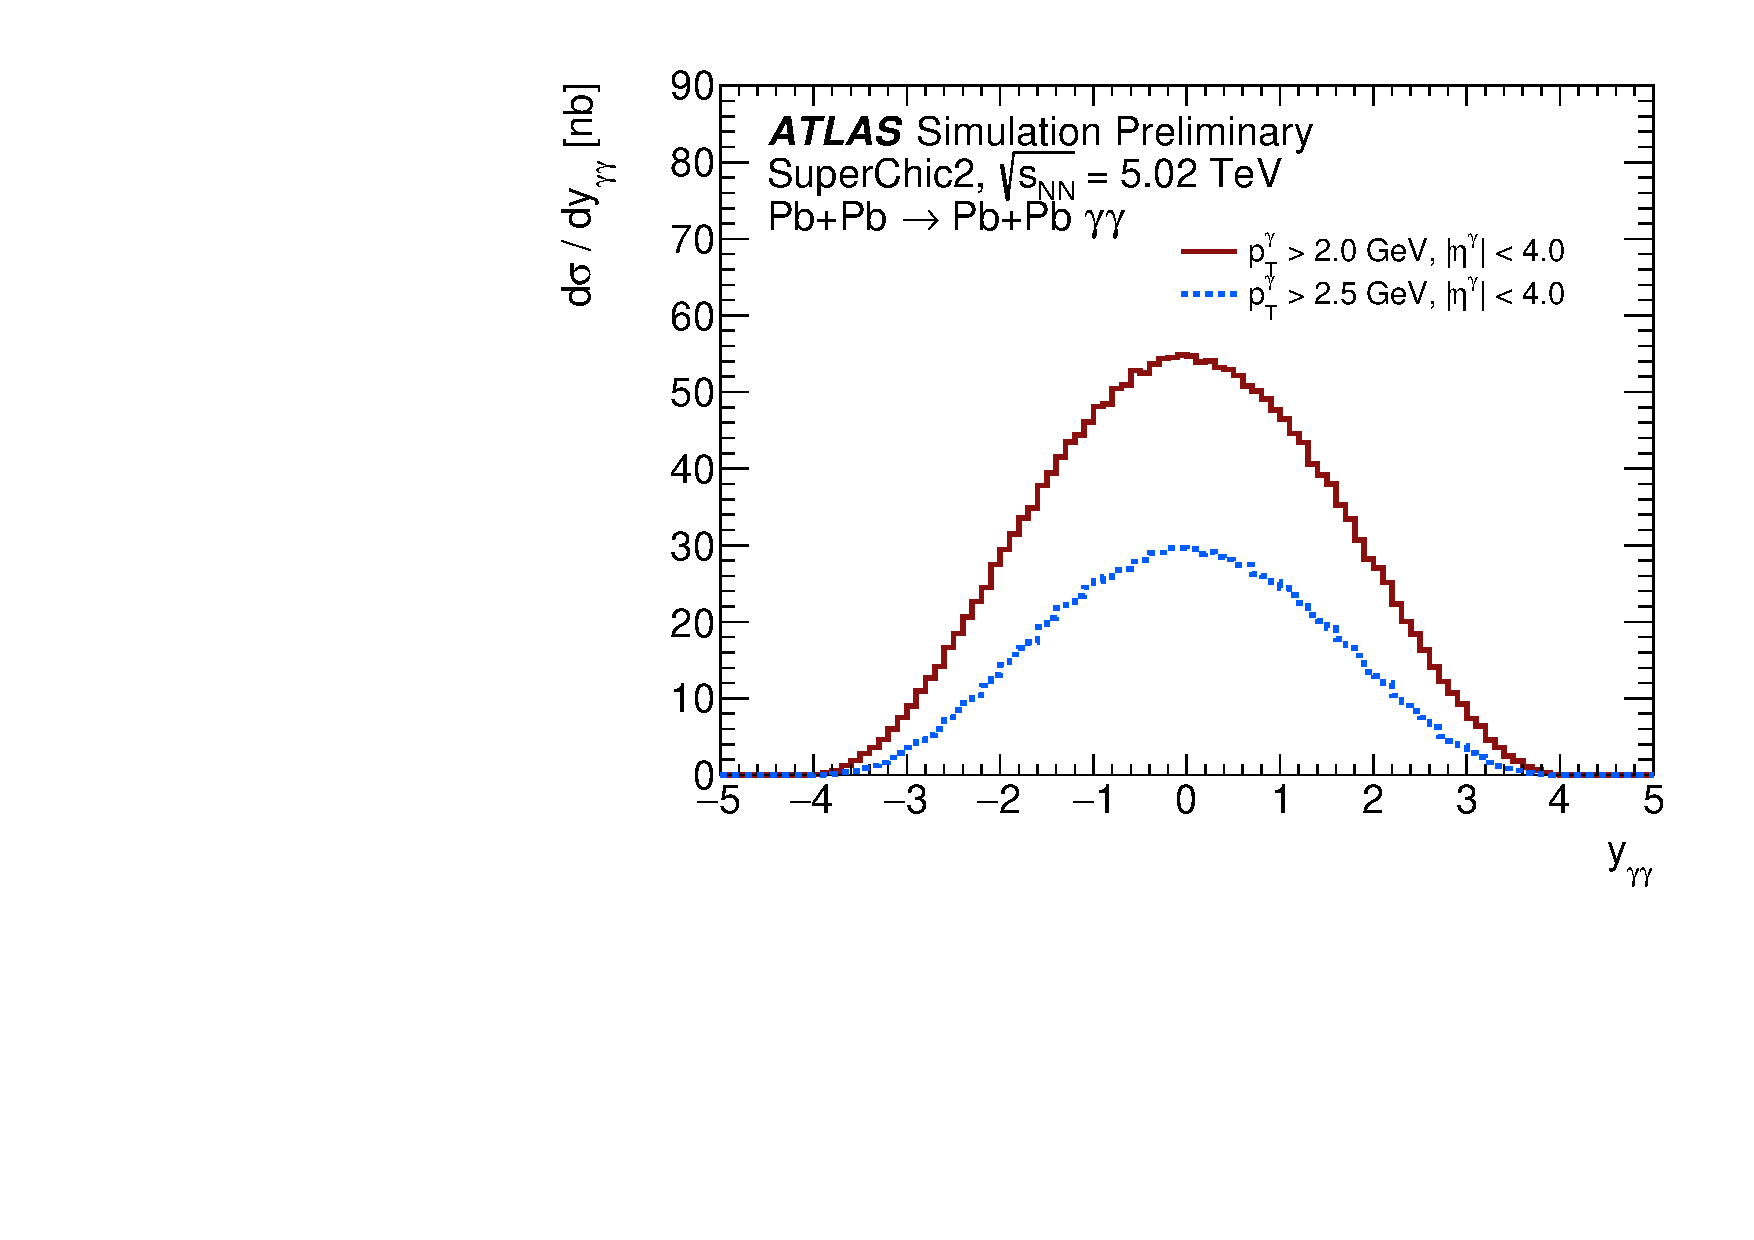
\includegraphics[width=0.49\linewidth]{\main/beyond/fig/fig_02.pdf}
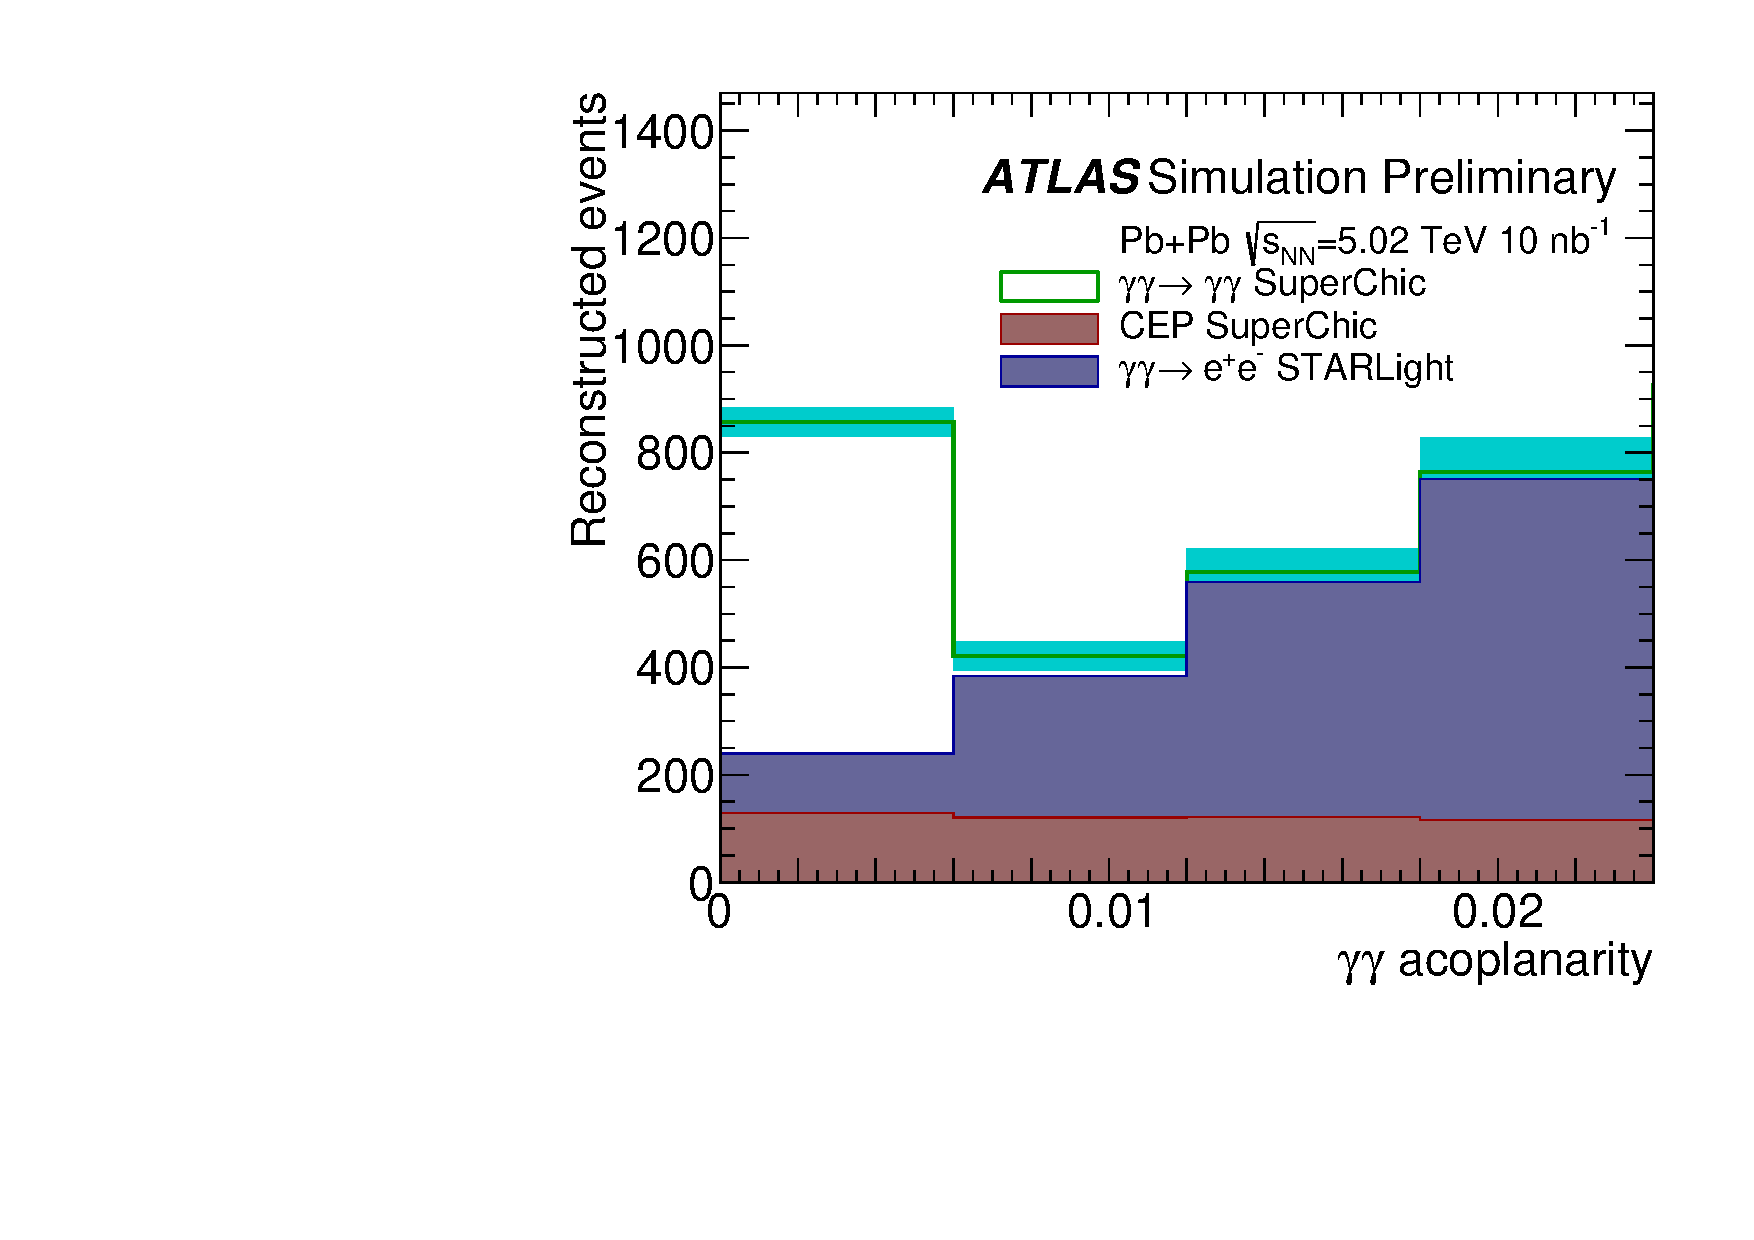
\includegraphics[width=0.425\linewidth]{\main/beyond/fig/fig_03a.pdf}
\caption{
(Left)~Predicted differential cross section as a function of the di-photon rapidity for LbyL scattering for photons with
$\pt^{\mathrm{\gamma}}>2.5$~GeV~(dashed) or $\pt^{\mathrm{\gamma}}>2.0$~GeV~(solid), and
$|\eta^{\mathrm{\gamma}}|<4$ extracted from SuperChic~\cite{Harland-Lang:2018iur}.
(Right) Detector-level acoplanarity distribution of the di-photon system for photons from the LbyL signal and background processes in
  5.02~TeV Pb--Pb collisions with an integrated luminosity of
  $10~\mathrm{nb}^{-1}$. The shaded band in cyan represents expected statistical uncertainties.
}
\label{fig:lbyl}
\end{figure}
%-------------------------------------------------------------------

The LbyL process can also be studied at lower di-photon masses. The differential cross sections as a function of the di-photon mass can be evaluated taking into account acceptance of the ALICE experiment, i.e. pseudorapidity limited to $|\eta^{\mathrm{\gamma}}|<0.9$ or in the forward region defined by $2<\eta^{\mathrm{\gamma}}<4.5$ in the LHCb experiment, and relatively low energies of outgoing photons~\cite{Abelev:2014ypa}. At lower energies~($W_{\mathrm{\gamma\gamma}} <$ 4~GeV) meson resonances~\cite{Klusek-Gawenda:2018ijg} may play an important role in addition to the Standard Model box diagrams~\cite{dEnterria:2013zqi,Klusek-Gawenda:2016euz} or double photon fluctuations into light vector mesons~\cite{Klusek-Gawenda:2016euz} or two-gluon exchanges~\cite{Klusek-Gawenda:2016nuo}.
%-------------------------------------------------------------------
\begin{figure}[!h]
        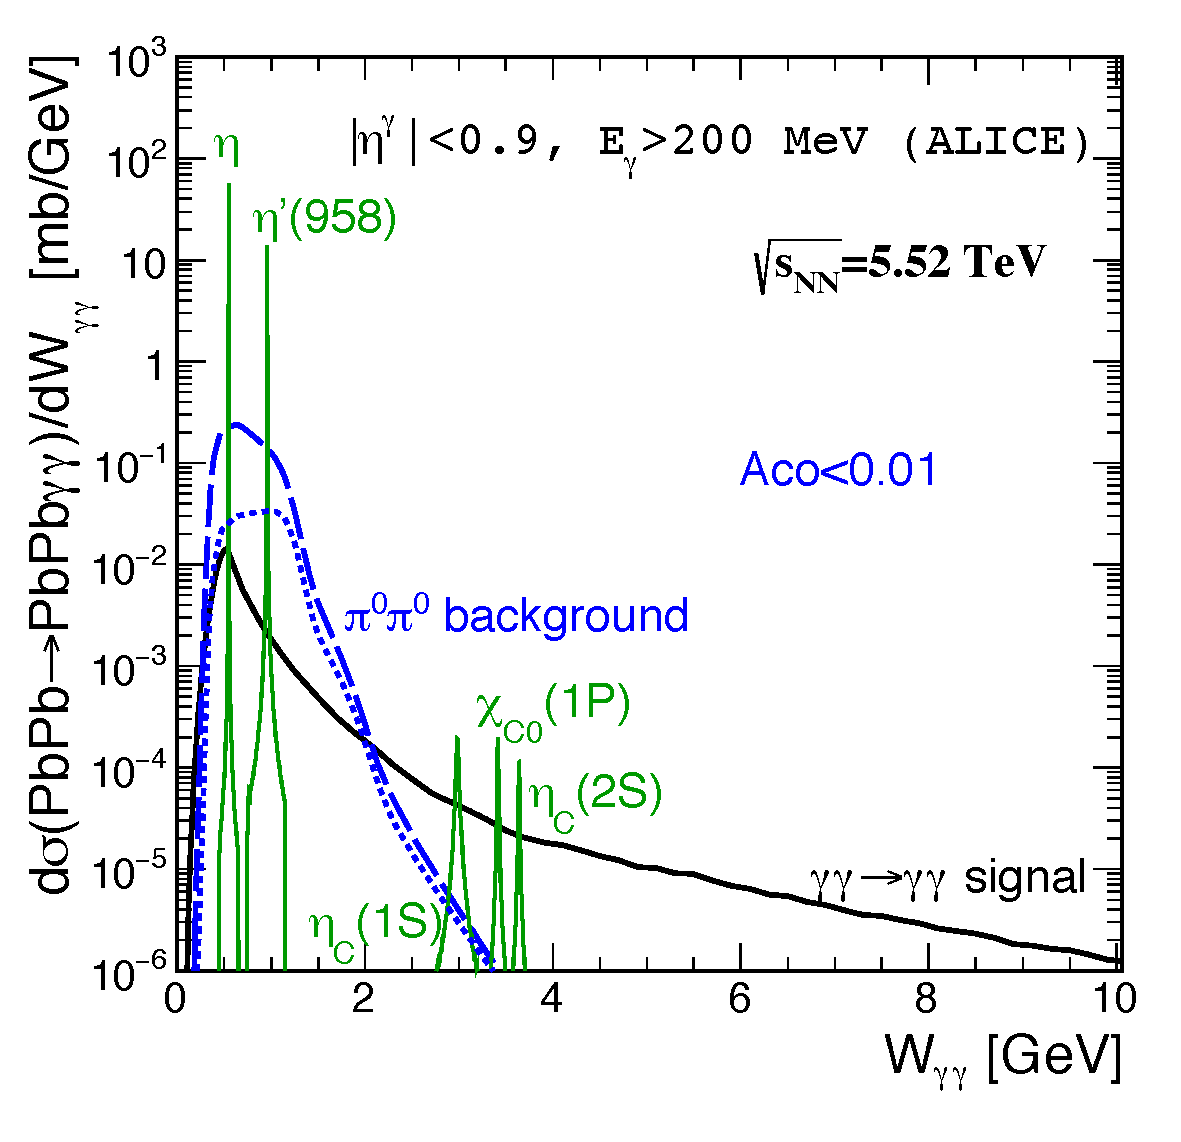
\includegraphics[scale=0.375]{\main/beyond/fig/dsig_dW_LbL_Pb_ALICE_aco001.pdf}%
        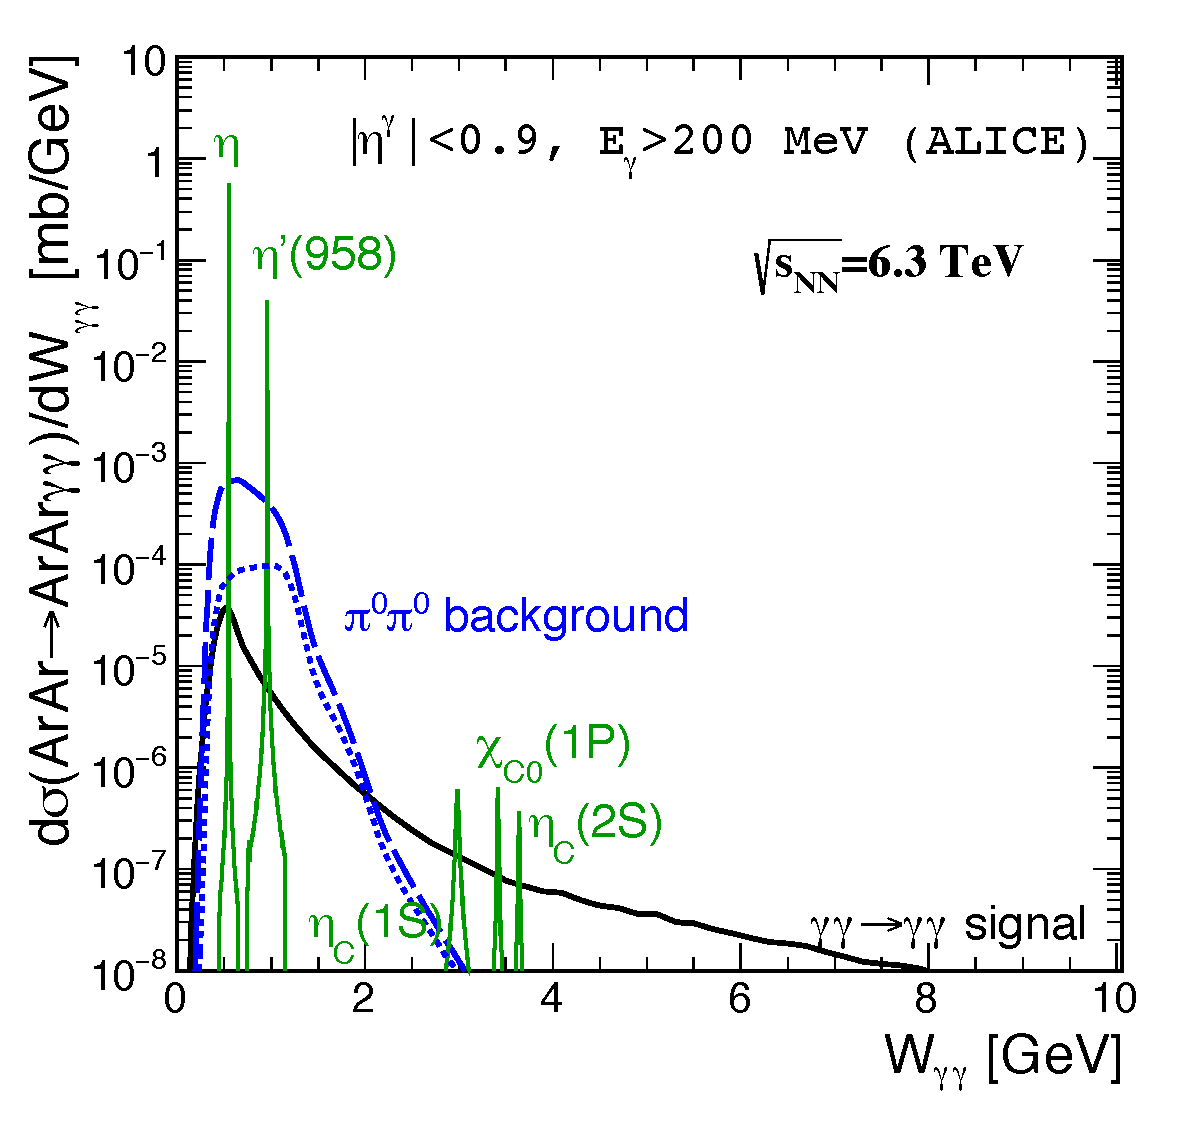
\includegraphics[scale=0.375]{\main/beyond/fig/dsig_dW_LbL_Ar_ALICE_aco001.pdf}\\
        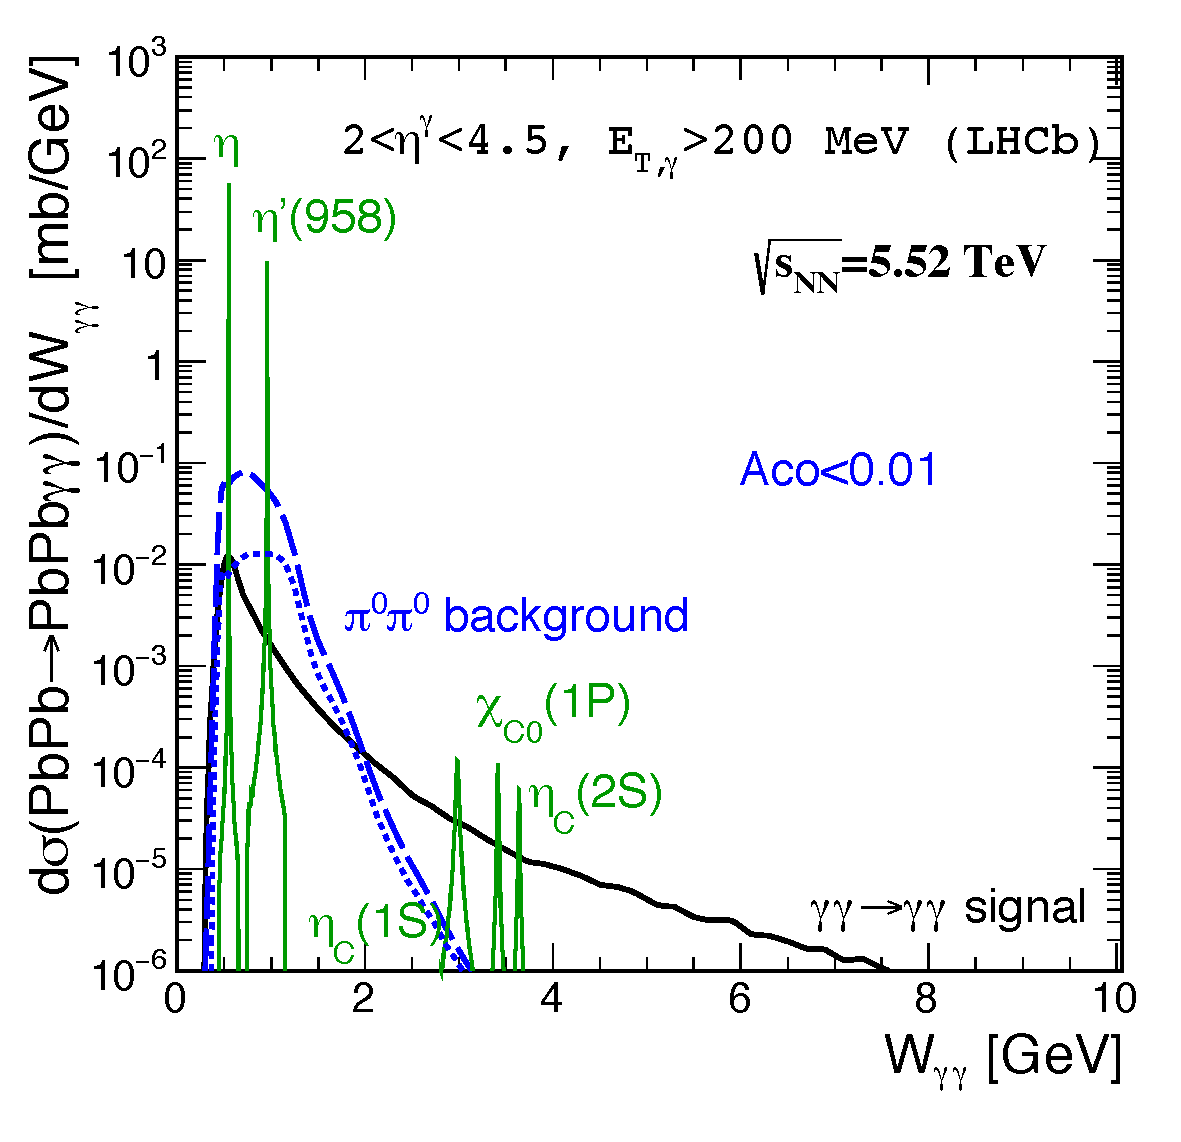
\includegraphics[scale=0.375]{\main/beyond/fig/dsig_dW_LbL_Pb_LHCb_aco001.pdf}%
        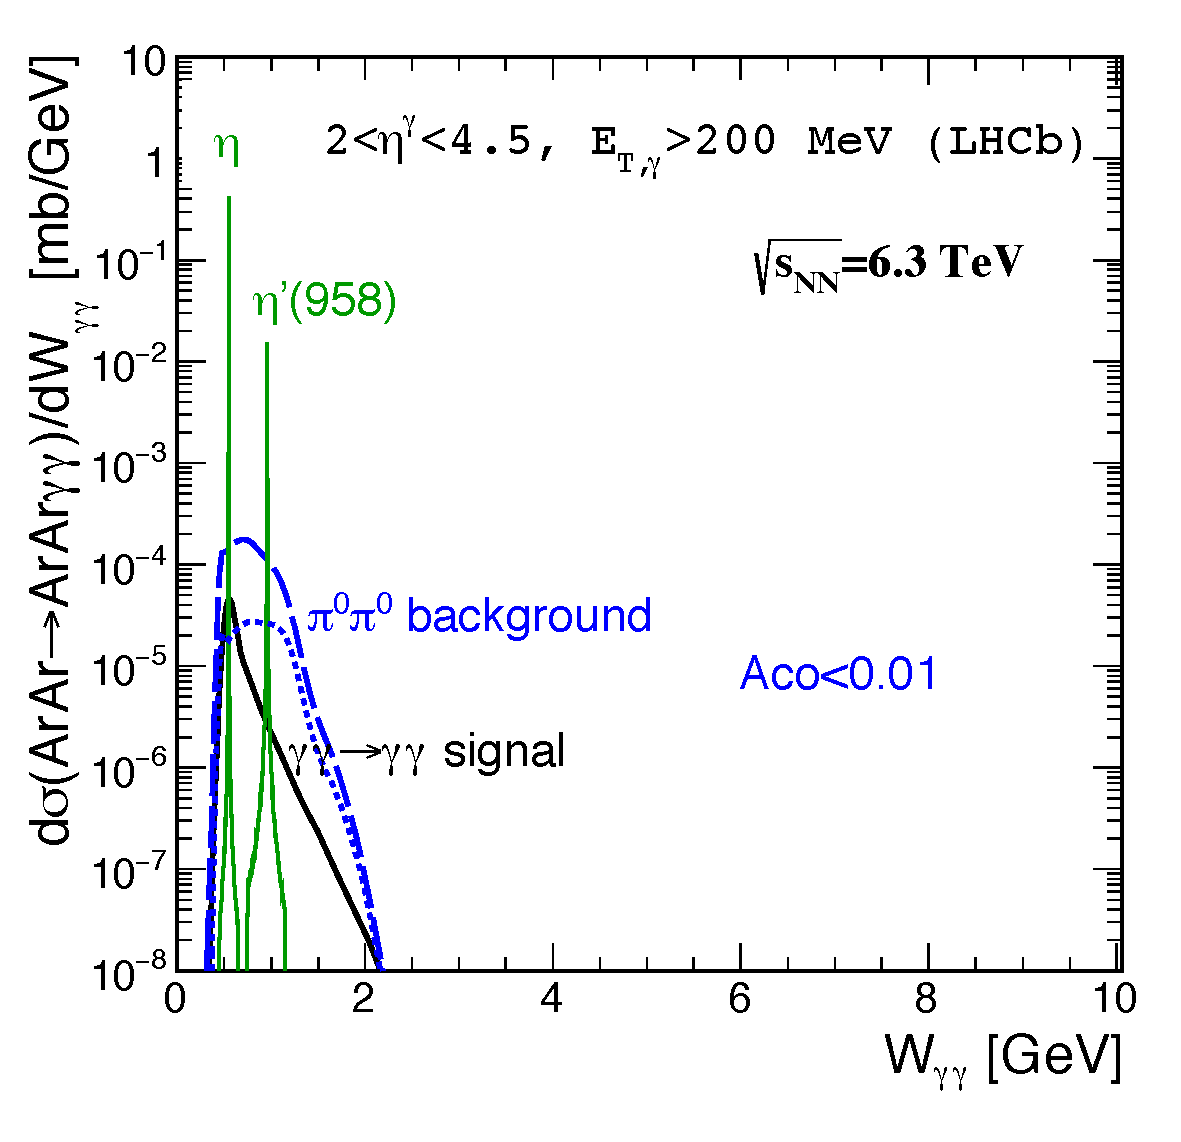
\includegraphics[scale=0.375]{\main/beyond/fig/dsig_dW_LbL_Ar_LHCb_aco001.pdf}
        \caption{
                Di-photon invariant mass distributions for Pb--Pb collisions at $\sqrt{s_{\mathrm{NN}}}$=5.52\,TeV~(left) and Ar--Ar collisions at $\sqrt{s_{\mathrm{NN}}}$=6.3\,TeV~(right) for ALICE at mid-rapidity~(top) and LHCb at forward pseudorapidity~(bottom). The $\mathrm{\pi^0\pi^0}$ background is shown with the acoplanarity requirement of 0.01~(dotted line) and also without it~(dashed line).}
        \label{fig:lbyl_alice}
\end{figure}
%-------------------------------------------------------------------
Figure~\ref{fig:lbyl_alice} shows predictions for LbyL and background processes in the ALICE and LHCb experiments with photon acceptance in $|\eta^{\mathrm{\gamma}}|<0.9$ and $E_{\mathrm{\gamma}}$ > 200~MeV~(top panel) or $2<\eta^{\mathrm{\gamma}}<4.5$ and $E_{\mathrm{T,\gamma}}$ > 200~MeV~(bottom panel), respectively, for two systems: Pb--Pb collisions at 5.52~TeV~(left panel) and Ar--Ar collisions at 6.3~TeV~(right panel). Presented results include the effect of the experimental energy resolution~\cite{Acharya:2018yhg,Govorkova:2015vqa}. The black-solid lines depict the LO QED fermionic box mechanism with leptons and quarks. Presented results for the $\mathrm{\gamma\gamma\to\gamma\gamma}$ process are in agreement with calculations from Refs.~\cite{Jikia:1993tc,Bern:2001dg,Bardin:2009gq}. The green-solid lines show nuclear results for the $s$-channel $\mathrm{\gamma\gamma}\to$pseudoscalar/scalar/tensor resonances that contribute to the LbyL process.
In the present analysis, $\eta$, $\eta'(958)$, $\eta_c(1S)$, $\eta_c(2S)$, $\chi_{c0}(1P)$ mesons are considered.
Their masses, total widths and branching ratios are taken from the PDG~\cite{Patrignani:2016xqp}.
The dominant background from the $\mathrm{\gamma\gamma\to\pi^0\pi^0}$
process is depicted by the blue lines. It becomes non-negligible only when one photon from each $\mathrm{\pi^0\to\gamma\gamma}$ decay is reconstructed in the detector. Two scenarios with and without the acoplanarity requirement of 0.01 are considered. The acoplanarity requirement reduces this background contribution by about 10\%.
The experimental data for the $\mathrm{\gamma\gamma\to\pi\pi}$ elementary cross section were very well described in Ref.~\cite{Klusek-Gawenda:2013rtu}.
There simultaneously the total cross section and angular distributions for both charged and neutral pions are shown.
Following Ref.~\cite{Klusek-Gawenda:2013rtu}, here nine resonances,
$\mathrm{\gamma\gamma\to\rho^\pm\to\pi^0\pi^0}$ continuum, Brodsky-Lepage and hand-bag mechanism are included. Figure~\ref{fig:lbyl_alice} shows that pionic background dominates at low invariant di-photon mass~(below 2~GeV).
In the same energy region, one can observe a very clear dominance of
$\mathrm{\eta}$, $\mathrm{\eta'(958)}$ mesons over boxes and background.
The inclusion of energy resolution has a significance mainly at
$\mathrm{\gamma\gamma\to\eta,\eta'\to\gamma\gamma}$ resonance scattering.
This contribution is supposed to be measured with good precision.
%However, the resonance signal is modified including experimental energy resolution and a peak is about one order of magnitude smaller than without experimental resolution but the total cross section is of course still the same.
These results suggest that both ALICE and LHCb Collaborations could measure LbyL scattering for $W_{\mathrm{\gamma\gamma}}>$ 2~GeV in Pb--Pb collisions. The cross sections are about two orders of magnitude lower in the Ar--Ar system due to smaller electric charge associated with argon beams. Assuming integrated luminosities of $3.0-8.8$~$\mathrm{pb^{-1}}$ in a dedicated Ar--Ar run, the LbyL production cross section leads to 1460-4280 signal events for ALICE and 11-34 events for LHCb in a range of $W_{\mathrm{\gamma\gamma}}>2$~GeV. A background contribution from $\mathrm{\gamma\gamma\to\pi^0\pi^0}$ is at the level of 20\% for ALICE and 134\% for LHCb in this region.


Axions and ALP are fundamental components of extensions of the Standard Model, occurring in most solutions of the strong CP problem~\cite{Peccei:1977hh,PhysRevLett.38.1440}. Recently an increasing interest has been paid to ALP masses
above 1~GeV~\cite{Bauer:2017ris,Mimasu:2014nea,Jaeckel:2015jla,Knapen:2016moh,Brivio:2017ije}. In particular the Higgs discovery has set spin zero particles in the spotlight of searches for new physics, with scalar and pseudo-scalar particles (elementary or not) as heralds of new phenomena. An interesting feature is that ALP (generically labelled as $\mathrm{a}$ in the following) in this mass range would induce an anomalous contribution to the LbyL, via the reaction:
$\mathrm{\gamma \gamma \rightarrow a \rightarrow \gamma \gamma}$,
under the condition that the magnitudes of the EM fields associated
with the incident photon are large enough, typically $\left|\vec{E}\right| >10^{18}$~V/m.
This has triggered  the study presented in Ref.~\cite{Knapen:2016moh},
and then in Ref.~\cite{Knapen:2017ebd} using the recent observation of LbyL scattering published by the ATLAS experiment in Pb--Pb collisions~\cite{Aaboud:2017bwk}, where the electric field produced by the ultra-relativistic Pb is of the order of $10^{25}$~V/m (thus satisfying the above condition).

The potential of ALP searches in UPC Pb--Pb collisions is studied using detector-level quantities after the LbyL selection requirements are imposed. The overall selection efficiency (times acceptance) relative to generated events increases from about $40$\% to $65$\% for ALP masses ranging from $7$~GeV to $80$~GeV. Also, the mass resolution varies from $0.5$~GeV at low masses (below $15$~GeV) up to $1$~GeV for larger masses. In the left panel of Figure~\ref{fig:alp} the expected mass distributions for three ALP signal mass values, and the main background from LbyL normalised to integrated luminosity of 10~$\mathrm{nb}^{-1}$ are shown. In this study, other sources of backgrounds are neglected, since they have been found to be small in the LbyL measurement~\cite{Aaboud:2017bwk}. The invariant mass distribution is used as the discriminating variable, with bin widths comparable to the expected resolution of a narrow resonant signal.
Upper limits are set on the product of the production cross section of
new resonances and their decay branching ratio into $\mathrm{\gamma\gamma}$. Exclusion intervals are derived using the CLs method~\cite{Read:2002hq} in the asymptotic approximation. The limit set on the signal strength $\mu$ is then translated into a limit on the signal cross section times branching ratio as presented in the right panel of Figure~\ref{fig:alp}.
%-------------------------------------------------------------------
\begin{figure}[!htbp]
\centering
  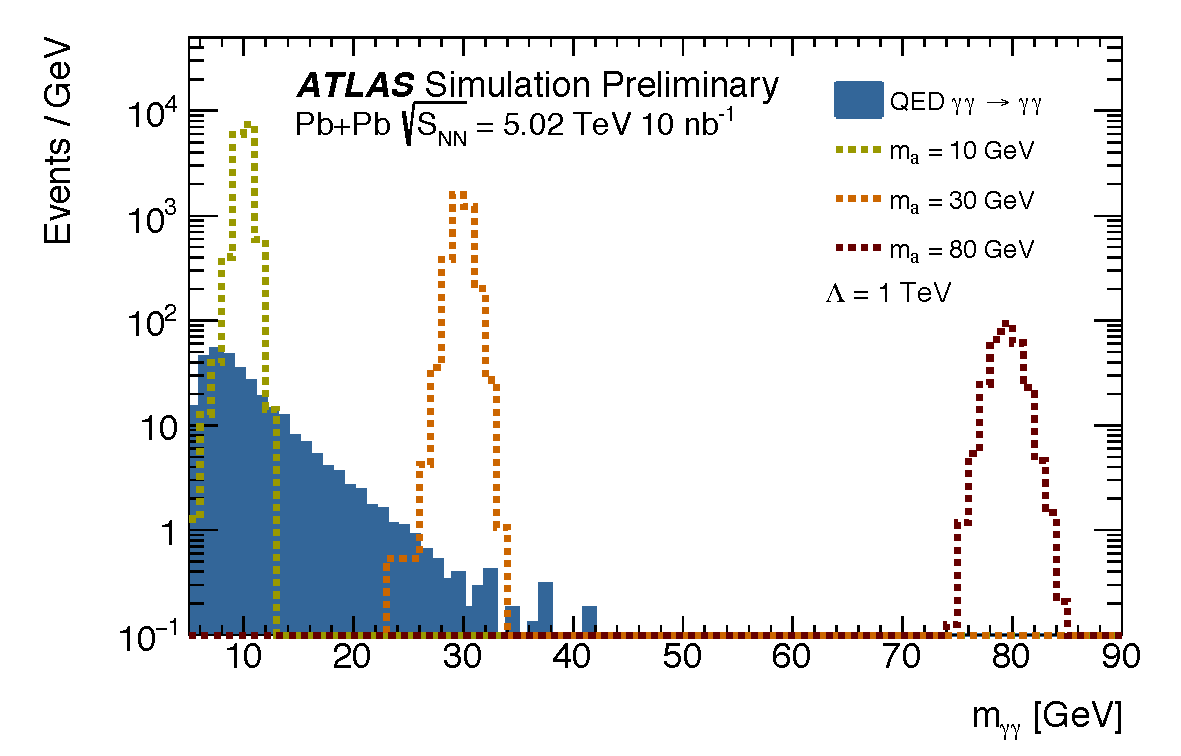
\includegraphics[scale=0.45]{\main/beyond/fig/fig_04.pdf}
  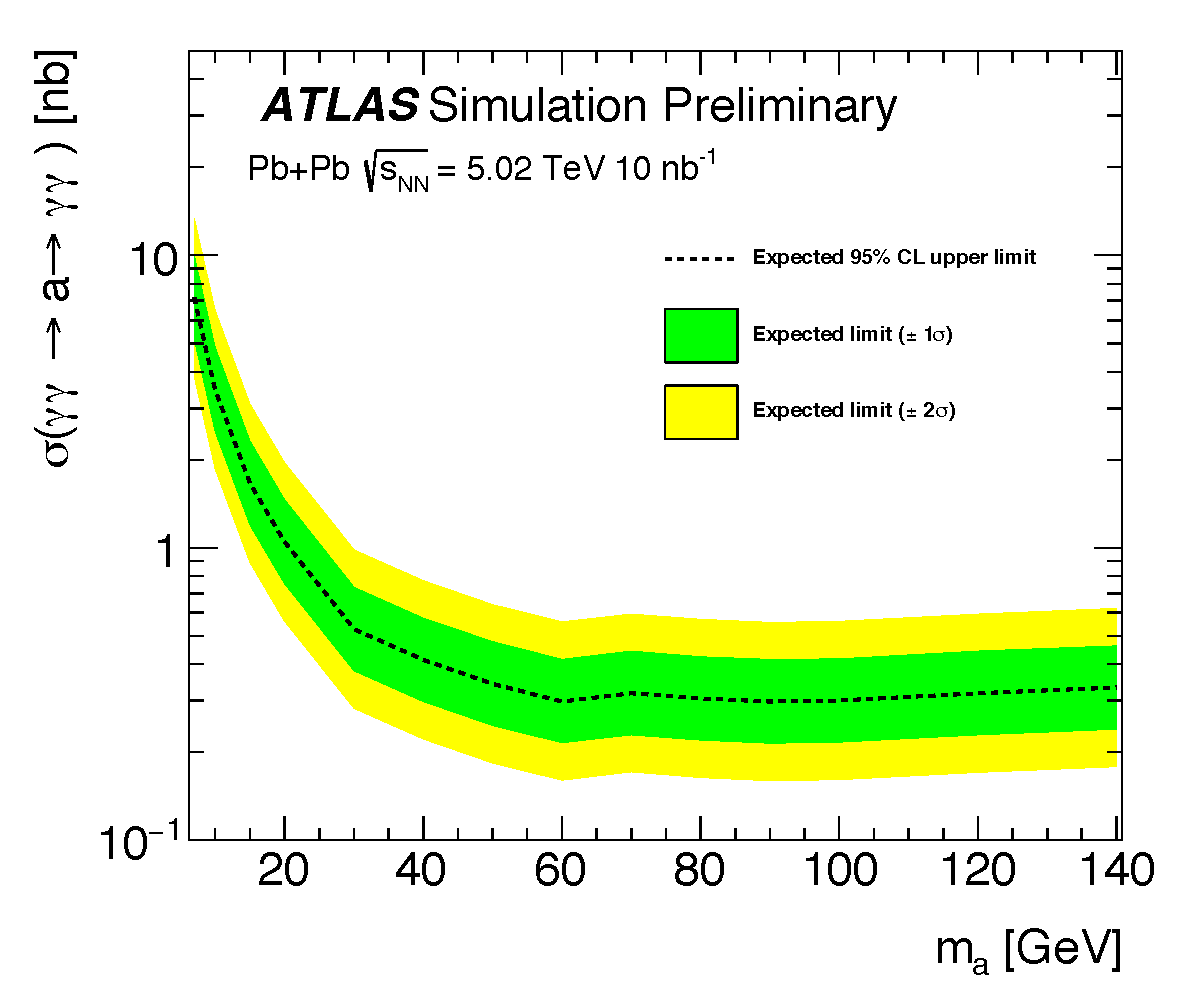
\includegraphics[scale=0.34]{\main/beyond/fig/fig_05a.pdf}
  \caption{(Left)~Mass distribution for the ALP signal
  shown for three values of the ALP mass: $m_\mathrm{a}=10, 30$ and
  $80$~GeV~(in red). Also shown (in blue) the LbyL background~(see
  text). All ALP mass points are generated with $\Lambda = 1$~TeV which follows a convention defined in Ref.~\cite{Knapen:2016moh}.
  (Right)~Expected $95$\% CLs upper limits on $\sigma_{\mathrm{a\rightarrow \gamma \gamma}}$.}
  \label{fig:alp}
\end{figure}
%-------------------------------------------------------------------

In Figure~\ref{fig:alp-lambda-limits} two exclusion limits on the coupling along with the existing exclusion limits from the compilation presented in Ref.~\cite{Baldenegro:2018hng} are presented. The LHC 10~nb$^{-1}$ limit is derived using the analysis described above at $\sqrt{s_{\mathrm{NN}}}=5.02$~TeV. The LHC 20~nb$^{-1}$ limit is established using a combined analysis of the ATLAS and CMS data assuming similar acceptance and photon performance in the two experiments and energy of $\sqrt{s_{\mathrm{NN}}}=5.52$~TeV of the Pb--Pb system.
Sensitivity of these analyses covers the range in ALP masses between $7$~GeV and $140$~GeV, where the previous analysis~\cite{Knapen:2016moh} is also shown~(labelled as ATLAS 2016 in the figure).

%-------------------------------------------------------------------
\begin{figure}[!htbp]
\centering
  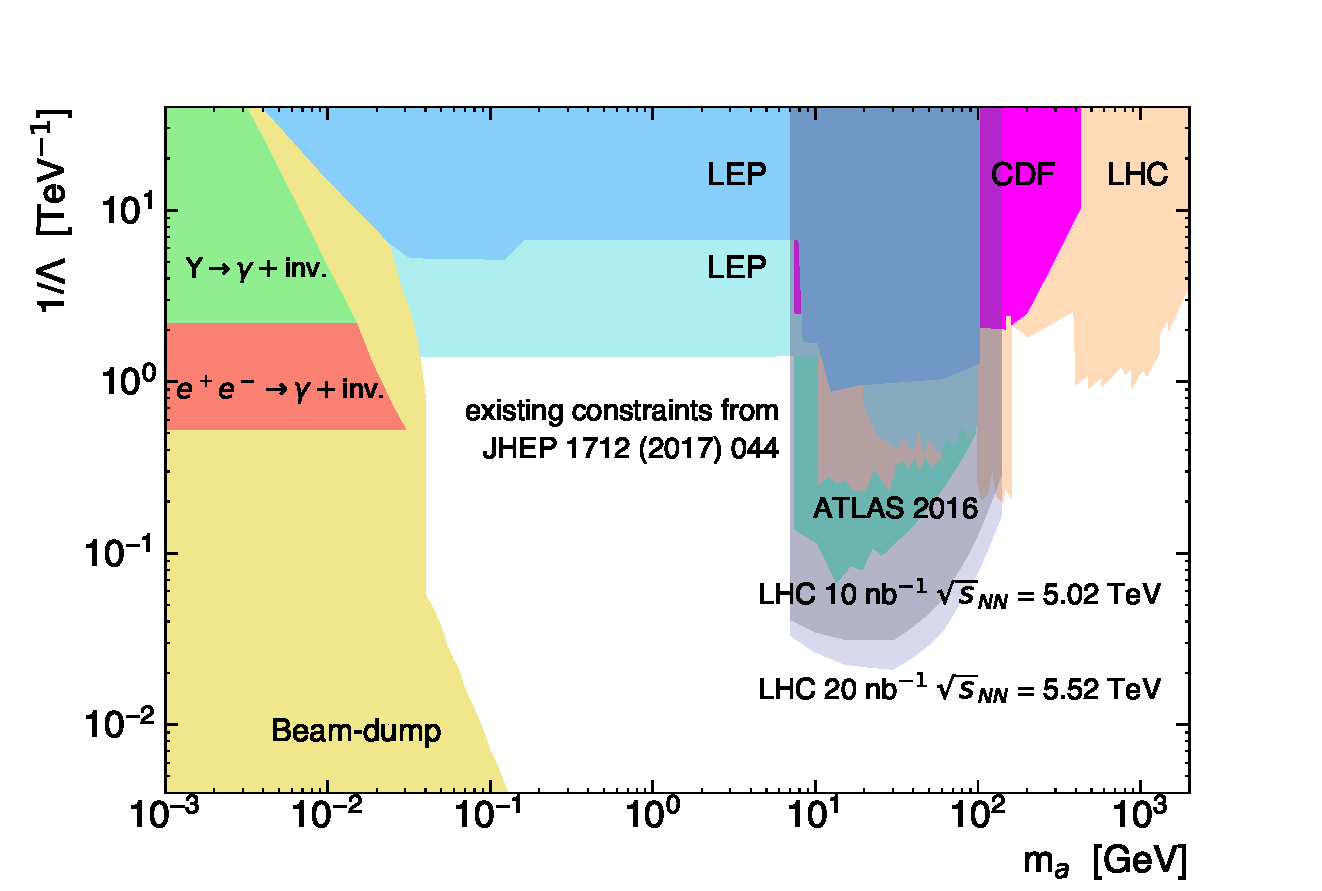
\includegraphics[scale=0.7]{\main/beyond/fig/ALPLimits_atlas_cms.pdf}
  \caption{Compilation of exclusion limits obtained by different experiments~(see text).
  ATLAS 2016 represents the exclusion limit derived from the recent LbyL cross section measured in Pb--Pb collisions by ATLAS.
  In dark grey, LHC 10~nb$^{-1}$ is shown corresponding to the analysis described in the text. Also in light grey, the LHC 20~nb$^{-1}$ limit for $\sqrt{s_{\mathrm{NN}}}=5.52$~TeV is presented. A more complete version of the existing constraints on ALPs masses versus coupling, including the constraints in the sub meV range from astrophysical observations and
  from dedicated experiments such as CAST can be found in Ref.~\cite{Bauer:2017ris}.}
  \label{fig:alp-lambda-limits}
\end{figure}
%-------------------------------------------------------------------

